\documentclass[10pt,twocolumn,letterpaper]{article}

\usepackage{cvpr}
\usepackage{times}
\usepackage{epsfig}
\usepackage{graphicx}
\usepackage{amsmath}
\usepackage{amssymb}

% Include other packages here, before hyperref.

% If you comment hyperref and then uncomment it, you should delete
% egpaper.aux before re-running latex.  (Or just hit 'q' on the first latex
% run, let it finish, and you should be clear).
\usepackage[breaklinks=true,bookmarks=false]{hyperref}
\usepackage{enumerate}

\newtheorem{definition}{Definition}[section]
\newtheorem{theorem}{Theorem}[section]
\newtheorem{proposition}{Proposition}[section]
\newtheorem{lemma}{Lemma}[section]
\newtheorem{corollary}{Corollary}[section]

\cvprfinalcopy % *** Uncomment this line for the final submission

\def\cvprPaperID{****} % *** Enter the CVPR Paper ID here
\def\httilde{\mbox{\tt\raisebox{-.5ex}{\symbol{126}}}}

% Pages are numbered in submission mode, and unnumbered in camera-ready
%\ifcvprfinal\pagestyle{empty}\fi
\begin{document}

%%%%%%%%% TITLE
\title{A Survey on Supervised Learning}

\author{Lanxiao Bai\\
University of Illinois at Urbana-Champaign\\
{\tt\small lbai5@illinois.edu}
% For a paper whose authors are all at the same institution,
% omit the following lines up until the closing ``}''.
% Additional authors and addresses can be added with ``\and'',
% just like the second author.
% To save space, use either the email address or home page, not both
%\and
%Second Author\\
%Institution2\\
%First line of institution2 address\\
%{\tt\small secondauthor@i2.org}
}

\maketitle
%\thispagestyle{empty}

%%%%%%%%% ABSTRACT
\begin{abstract}
   As a powerful tool for classification and regression, supervised learning recently captured attention of both academia and industry thanks to the success of Deep Learning algorithms since AlexNet's\cite{Krizhevsky:2012:ICD:2999134.2999257} excellent performance in ImageNet. But long before that, there are also a lot of methods and algorithms that are as well widely used in different fields. In this work, we provides a full exploration of supervised learning methods and we hope that it will provide a better understanding on the history and status quo of supervised learning and discuss some application of these methods.
\end{abstract}

%%%%%%%%% BODY TEXT
\section{Introduction}

Among all tasks of Machine Learning(ML) and Data Mining, two of the most significant and the most researched are classification and regression. As we enter the era of data, we are drowning in so much information so that it is very hard for human to conduct manual search for valuable knowledge and other data with meaningful structures. For an instance, there are about 1 trillion web pages\footnote{http://googleblog.blogspot.com/2008/07/we-knew-web-was-big.html} on the Internet, and in each page, there are also great amount of texts, images, videos and some other types of data and that's just the potential information we have active access to.

On the other hand, thanks to the digital notification services, RSS softwares and emails, we also can be bombarded with hundreds even thousands of fragments of information each day, but among them all, we are interested only very small part of them. If we have to manually pick and consume these data every day, a lot of time will be wasted. In other words, it is important that we have an efficient system of classification that can automatically handle all these mixed information. In fact, classification systems are already widely used to construct anti-SPAM and recommendation systems\cite{murphy_2013}.

%-------------------------------------------------------------------------
\subsection{Challenges}

Although methods of supervised learning is well-researched, applying appropriate algorithms to corresponding problems is still hard and some challenges appear in the process of deployment of these methods:
\begin{enumerate}[(i).]
	\item \textbf{Curse of Dimensionality.} When the number of attributes of data is low, it is easy to analyze the contribution of each attribute to the problem and picking the useful attributes that lead to maximization of performance. However, as the number of possible combinations grows exponentially, it becomes very hard to examine if certain attributes are useful\cite{goodfellow_bengio_courville_2017}.
	\item \textbf{Bias-Variance Tradeoff.} Considering mean squared error (MSE)
	\begin{align}
		&MSE = \mathbb{E}[(\hat{\theta}_m - \theta) ^ 2]\nonumber\\
		&\phantom{MSE} = Bias(\hat{\theta}_m)^2 + Var(\hat{\theta}_m)\cite{goodfellow_bengio_courville_2017}
	\end{align}
	
	we see that both the bias and variance of a model contribute to the generalization error, so it is inherently hard to choose a suitable number of parameters. While too many parameters will lead to overfitting, which means that the performance of model on training dataset is much higher than that on testing (unseen) dataset and vice versa\cite{goodfellow_bengio_courville_2017} as shown in Figure 1\cite{bishop}.
	
	\begin{figure}[h]
		\begin{center}
		   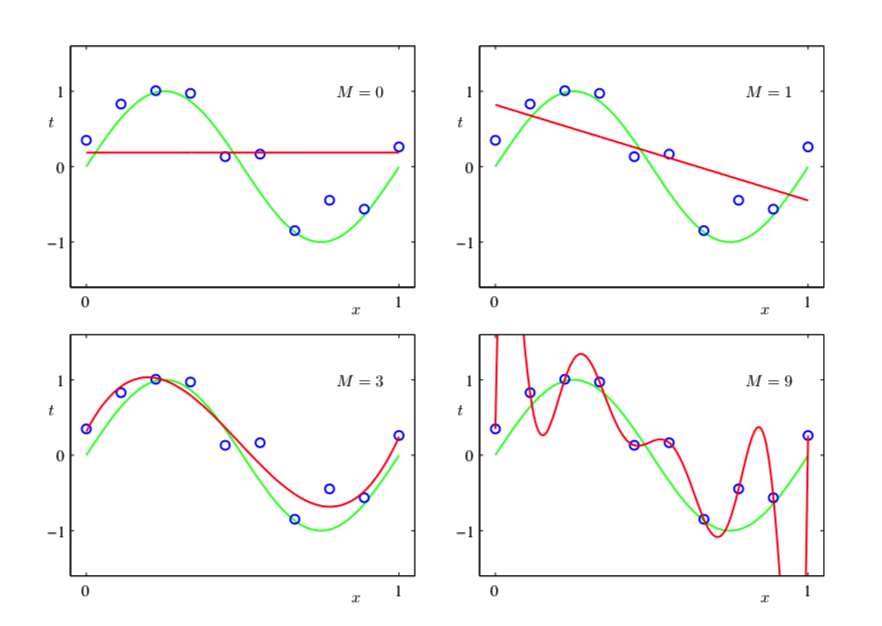
\includegraphics[width=0.8\linewidth]{./images/overfitting.png}
		\end{center}
   \caption{Fitting dataset with different models}
\end{figure}
\end{enumerate}

\subsection{Our contribution}
	Our survey provides the following contribution:
	\begin{enumerate}[(i).] 
		\item We examine the similarities and differences of methods and algorithms we have for supervised learning and provide a taxonomy of approaches to supervised learning and how they fit problems in different scenes.
		\item We provide a detailed and comprehensive analysis on various kinds of supervised learning models, specifically, on the properties of the models and how these properties can be utilized or how the models can be modified to handle the challenges we mentioned above.
	\end{enumerate}

\subsection{Organization of the Survey}
In Section 2, we will introduce the definition required to understand and analysis the models theoretically. Section 3 introduces the classification of the supervised learning methods we have, and Section 4-6 will cover details of approaches in each category. And in Section 7, we will talk about some popular application of supervised learning in some domains.

%-------------------------------------------------------------------------
\section{Definition of Tasks}

\subsection{What is Supervised Learning?}

\begin{definition}
	Suppose we have a labeled dataset $\mathcal{D} = \{x_i, y_i\}$ in which $x_i$ is called instances or inputs and $y_i$ is called labels that represent categories, our goal is to find a function $h$ which, ideally, have 
		\[h(x_i) = y_i\]
		
		for all $x_i \in \mathcal{D}$.
\end{definition}

\subsection{What is a good model?}

In order to evaluate the performance of our models, we define two kinds of metrics.

\begin{definition}[Risk]
	Risk function $R$ is a function that satisfy the following rules:
	\begin{itemize}
		\item $R(h, \mathcal{D}) = 0$ if $h(x_i) = y_i$ for all $(x_i, y_i) \in \mathcal{D}$
		\item $R(h, \mathcal{D})$ grows as the number of $(x_i, y_i)$ that $h(x_i) \neq y_i$ increases
	\end{itemize}
\end{definition}

Vice versa, we have the utility function defined as following
\begin{definition}[Utility]
	Utility function $U$ is a function that satisfy the following rules:
	\begin{itemize}
		\item $U(h, \mathcal{D}) = 0$ if $h(x_i) \neq y_i$ for all $(x_i, y_i) \in \mathcal{D}$
		\item $U(h, \mathcal{D})$ grows as the number of $(x_i, y_i)$ that $h(x_i) = y_i$ increases
	\end{itemize}
\end{definition}

In order to design an appropriate metric function, domain knowledge and robustness need to be considered.

In order to evaluate the generalization capacity of model, we define

\begin{definition}[Generalization Risk]
	\[R_G = |R(h_n, \mathcal{P}) - R(h_n, \mathcal{D}_n)|\]
	
	in which $\mathcal{P}$ is the population.
\end{definition}

A good model has high utility and low risk, and low generalization risk\cite{goodfellow_bengio_courville_2017}, which means that it does not only has good performance on training dataset, but also on testing unseen dataset.

\section{Taxonomy}
	There are many ways we can construct our model for supervised learning as shown in the table.
	
	\begin{center}
		\begin{tabular}{c || c}
			\hline
				Category & Algorithms\\
			\hline\hline
				Probabilistic Model & Naive Bayes, Logistic Regression\\
			\hline
				Logic based Model & Decision Tree, Random Forest, Boosting\\
			\hline
				Neural Network & Perceptron, Deep Learning\\
			\hline
				Kernel based Model & SVM, Kernelized Ridge Regression\\
			\hline
				Instance-based learning & kNN\\
			\hline
		\end{tabular}
	\end{center}

	Among these methods, statistical approaches is known for having an explicit underlying probability model\cite{kotsiantis2007supervised}, logical based approaches utilize certain logical rules to select correct labels, neural networks for now work as a black box that captures the features of given database and use backpropagation to adjust weights of neurons and kernel algorithms maps data into high-dimension spaces so that a hyper-plane can be determined to separate data with different labels.

%------------------------------------------------------------------------
\section{Probabilistic Models}
	Statistical learning algorithms provide a probability that an instance belongs in each class, rather than simply a classification\cite{kotsiantis2007supervised}, so that our goal is changed to estimating the parameters of the model, so that the likelihood function or a posterior can be maximized.
	
	\[w^* = \arg \max_{w} p(x \mid w),\footnote{Maximum Likelihood Estimation(MLE)}\]
	
	or
	
	\[w^* = \arg \max_{w} p(x \mid w)p(w),\footnote{Maximum A Posterior(MAP)}\]
	
	so that our classifier is
	
	\[\arg\max_k p(y_i = k \mid x_i, w)\]
\subsection{Naive Bayes}
	Naive Bayes is derived from the assumption that feature $x_i$ is conditionally dependent of every other feature $x_j \neq x_i$, so that
		\[p(\mathbf{x} \mid C) = \prod_{i} p(x_i \mid C)\]
		
	As a result, with Bayes' Theorem, we have
		\begin{align}
			&p(C_k \mid \mathbf{x}) = \frac{p(\mathbf{x} \mid C_k)p(C_k)}{p(\mathbf{x})}\nonumber\\
			&\phantom{p(C_k \mid \mathbf{x})} = \frac{p(C_k)\prod_{i} p(x_i \mid C_k)}{p(\mathbf{x}}\nonumber\\
			&\phantom{p(C_k \mid \mathbf{x})} = \frac{p(C_k)\prod_{i} p(x_i \mid C_k)}{\sum_j p(C_j)p(\mathbf{x} \mid C_j)}\nonumber
		\end{align}
		
	So that
	
	\[y = \arg\max_k \frac{p(C_k)\prod_{i} p(x_i \mid C_k)}{\sum_j p(C_j)p(\mathbf{x} \mid C_j)}\]
	
	One of the best known usage of Naive Bayes Classifier is Document classification. Assume that documents are drawn from a number of classes of documents, by calculating the word occurrence vector of texts, we can feed the data into the classifier and predict the category of the document. 
	
	In application, we can either apply it to a multi-class classification to predict the theme of given texts, so that we can recommend it to the user if their preference matches the prediction. We can also apply it to a binary classification task and predict if an incoming email is a spam and decide whether it should be filtered.
	
	The major advantage of the naive Bayes classifier is its short computational time for training\cite{kotsiantis2007supervised}. If a feature is numerical, we can discretize it during data pre-processing \cite{2003yang&webb} ,or it is also possible to use the normal distribution to calculate probabilities\cite{Bouckaert2004}.
	
	However, the conditionally independent assumption is almost always wrong, so that when in sophisticated learning tasks, it's accuracy is usually lower than other algorithms. There are various attempts to modify the model and improve its performance
\subsection{Linear Model and Logistic Regression}	
	Linear Model is the most common model in supervised learning\cite{murphy_2013}, not only because there are a lot of data that are linearly separable, but for the cases that data can not be perfectly separated, kernel tricks or nonlinear activation functions in Neural Networks can be used to introduce nonlinearity to the model.
	
	We commonly model the noise as a Gaussian distribution, so that the mean of the model is a hyper-plane.
	
	\[p(y \mid \theta, x) = \mathcal{N}(y \mid \mathbf{w}^T\mathbf{x}, \sigma^2)\]
	
	As mentioned above, one common way to estimate the parameters is to use Maximum Likelihood Estimation\cite{murphy_2013}.
	
	\begin{align}
	    & l(\theta) = \sum_{i = 1}^n \log \mathcal{N}(w^T, \sigma^2)\nonumber\\
	    & \phantom{l(\theta)} = \sum_{i = 1}^n-\frac{1}{2\sigma^2}(y_i - w^Tx_i) - \frac{1}{2}\log (2\sigma^2\pi)\nonumber
	\end{align}

Then \[\min_{w, \sigma^2} -l(\theta) = \min_{\sigma^2}\left[- \frac{1}{2}\log (2\sigma^2\pi) + \frac{1}{2\sigma^2} \min_w RSS(w)\right]\]

in which
	\[RSS = \frac{1}{2}||y - xw||^2_2 = \frac{1}{2}(y - xw)^T(y - xw)\]
	
	\begin{figure}[h]
			\begin{center}
				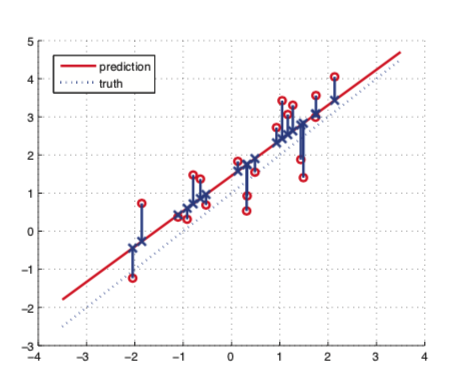
\includegraphics[width=0.8\linewidth]{images/linear}
				\caption{Linear least squares\cite{murphy_2013}}
			\end{center}
		\end{figure}

	There're several ways, the minimization can be done:
	\begin{itemize}
		\item Linear least squares, we try to minimize the sum of squared distances from each training point (denoted by a red circle) to its approximation\cite{murphy_2013}
		\item Maximum Likelihood Estimation
			\[\mathbf{w} = \arg\max_{\mathbf{w}} \log p(\mathbf{x} \mid \mathbf{w})\]
		\item Gradient Descent
			\[\mathbf{w}^{(t)} = \mathbf{w}^{(t - 1)} - \gamma \nabla l(\mathbf{w})\]
	\end{itemize}
	
	\begin{figure}[h]
			\begin{center}
				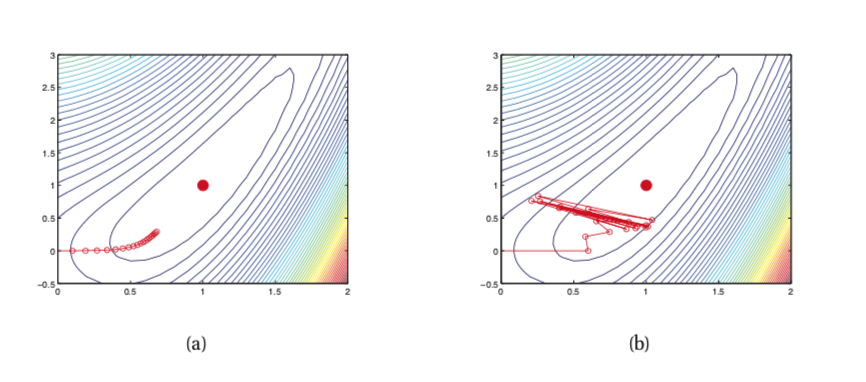
\includegraphics[width=0.9\linewidth]{images/gd}
				\caption{Gradient Descent\cite{murphy_2013}}
			\end{center}
		\end{figure}
	
	In the first two ways, we are able to get a closed form of estimation
	
	\[\mathbf{w}^* = (\mathbf{X}^T\mathbf{X})^{-1}\mathbf{X}^T\mathbf{y}\]
	
	In order to prevent this model from overfitting, regularization terms can be used to add punishment to the model if it does not satisfy some requirements, so that the loss function is now
	
	\[L(\mathbf{w}) = \frac{1}{N} \sum_{i = 1}^N (y_i - \mathbf{w}^T\mathbf{x}_i)^2 + \lambda_1 ||\mathbf{w}||_1 + \lambda_2 ||\mathbf{w}||_2^2\]
	
	We see that $l_2$ norm punishes weights that has too large magnitude and $l_1$ forces as many weights as possible to be zero\footnote{This means that $l_1$ norm can give us sparsity. In fact, $l_0$ norm gives the best sparsity, but that would make the optimization problem a NP problem to solve}.
	
	Similarly, we have the estimation of $\mathbf{w}$ to be
	
		\[\mathbf{w}^* = (\lambda\mathbf{I} + \mathbf{X}^T\mathbf{X})^{-1}\mathbf{X}^T\mathbf{y}\]
		
	this result can be derived from MAP as well, since regularization can also be regarded as prior distribution of $\mathbf{w}$\cite{bishop}.
	
	For classification tasks, we introduce sigmoid function\cite{alpaydin2004introduction}
		\[\sigma(x) = \frac{1}{1 + \exp(\mathbf{w}^T\mathbf{x})}\]
		
	and softmax function\cite{alpaydin2004introduction}
	
		\[f(x) = \frac{\exp(\mathbf{w}_j^T\mathbf{x})}{\sum_{k = 1}^K \mathbf{w}_k^T\mathbf{x}}\]
	
	to map vector to the probability an instance should be classified as class $k$ respectively for binary and muiticlass classification.
	
	In order to get weights that can minimize the loss function, other than gradient descent, we can also apply Stochastic Gradient Descent(SGD) 
	\[w = w - \frac{1}{n}\eta \sum_i \nabla l(w, x_i)\]
	
	The major advantage of SGD over GD is that, SGD take only part of the data(called a batch) to compute the gradient and iteratively update the weights. SGD also allows model to perform online learning, so the model can consistently evolve as new data flows in.\cite{alpaydin2004introduction} And this strategy is very effective in the case of large-scale machine learning problems\cite{bottou-bousquet-2008}.
	
	One significant challenge is that the loss function is almost never convex\cite{NIPS2016_6112}, which means that SGD only guarantees local minima, so the performance of SGD heavily relies on initialization.
	
	In high-dimensional space, the occasion is a little different. As the dimension goes up, the probability the gradient is zero in any direction become very low, but there are a lot of saddle points\cite{NIPS2016_6112}, and at those points the convergence will be very slow. Also, when the learning rate is fixed, if learning rate is too small, the training will suffer from painfully slow convergence; if learning rate is too large, the loss function will fluctuate around the minimum or even to diverge\cite{ruder_2017}.
	
	In order to overcome those flat areas in weight space, many strategies are designed.
	
	For areas like ravines, namely, areas where the surface curves much more steeply in one dimension than in another\cite{sutton:problems}, momentum is used to modify the direction of descent with the direction of last update
	
	\[v_t = \gamma v_{t - 1} + \eta \nabla_w L(w)\]
	
	and
	
	\[w = w - v_t\]
	
	\begin{figure}[h]
		\begin{center}
			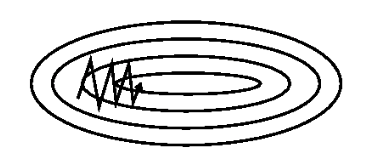
\includegraphics[width=0.9\linewidth]{images/without.png}
			\caption{SGD without momentum}	
		\end{center}
	\end{figure}
	
	\begin{figure}[h]
		\begin{center}
			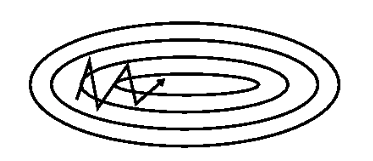
\includegraphics[width=0.9\linewidth]{images/with.png}
			\caption{SGD with momentum}	
		\end{center}
	\end{figure}
	
	Just blindly following the slope is usually unsatisfactory\cite{ruder_2017}, so that we have SGD to have a notion of where to slow down before the hill slopes up again. Nesterov accelerated gradient (NAG)\cite{nesterov} is able to give the momentum such prescience. NAG first makes a big jump in the direction of the previous accumulated gradient, measures the gradient and then makes a correction, which results in the complete NAG update\cite{ruder_2017}. 
	
	\begin{align}
		&v_t = \gamma v_{t - 1} + \eta \nabla_w L(w - \gamma v_{t - 1})\nonumber\\
		&w = w - v_t\nonumber
	\end{align}
	
	On the other hand, in order to handle the problem of learning rate scheduling, some other updating algorithms are invented. Adagrad\cite{Duchi:2011:ASM:1953048.2021068} adapts the learning rate to the parameters, performing larger updates for infrequent and smaller updates for frequent parameters, so that it greatly improved the robustness of SGD\cite{NIPS2012_4687} by excellently deal with sparse data.
	
	Geoffery Hinton proposed RMSProp in his lecture\footnote{http://www.cs.toronto.edu/~tijmen/csc321/slides/lecture\_slides\_lec6.pdf}, which can adaptive learning rate.
		
\section{Logic based Models}

\subsection{Decision Tree}
		By recursively splitting datasets for training based on some attributes of the datasets, the decision tree algorithm can partition the input space $\mathcal{X}$ into different regions, so that the all (or at least majority of) points $x_i \in \mathcal{X}_j$ has the same label $y$. RMSprop divides the learning rate by an exponentially decaying average of squared gradients\cite{ruder_2017}.
		
		\begin{figure}[h]
			\begin{center}
				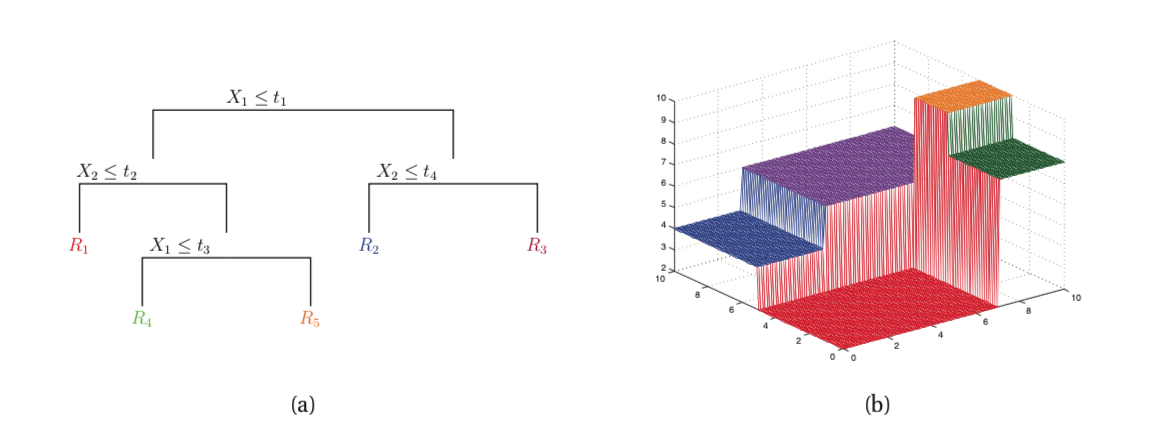
\includegraphics[width=0.9\linewidth]{images/classificationtree}
				\caption{Decision Trees\cite{murphy_2013}}
			\end{center}
		\end{figure}
    	
    	In order to increase the purity of each branch after splitting, there're several evaluation metrics to determine based on which attribute and the corresponding value can the post-split purity reaches the highest value. In general, there're several properties that the impurity metric $\phi$ should meet in order to be use:
    	
    	For simplicity, we consider the metric for binary classification, and let $p$ be the probability of a label if uniformly randomly picked, then
    	
    	\begin{enumerate}
    		\item $\forall p \in [0, 1], \phi(1/2, 1/2) \geq \phi(p, 1 - p)$
    		\item $\phi(0, 1) = \phi(1, 0) = 0$
    		\item $p$ is increasing on $[0, 1/2]$ and decreasing on $[1/2, 1]$
    	\end{enumerate}
    
    	These properties and be easily extend to $k$-ary classification, and some of the most commonly used methods are
    	\begin{itemize}
    		\item Entropy: $\phi(p) = -(p\log_2p + (1 - p)\log_2(1 - p))$
    		\item Gini index: $\phi(p) = 2p(1 - p)$
    	\end{itemize}
    	
    	\begin{figure}[h]
			\begin{center}
				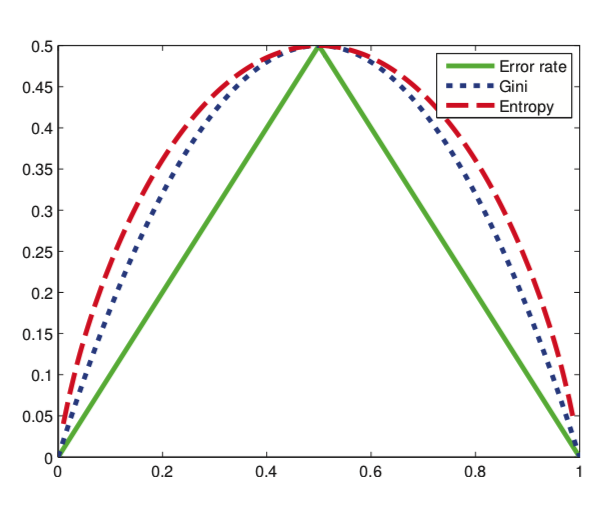
\includegraphics[width=0.8\linewidth]{images/impurity}
				\caption{Impurity measures\cite{murphy_2013}}
			\end{center}
		\end{figure}
		
		One problem of Decision Tree is that, when completely grown, a decision tree suffers seriously from overfitting. In order to prevent that, we can stop growing the tree if the decrease in the error is not su cient to justify the extra complexity of adding an extra subtree\cite{murphy_2013} or prune the fully grown tree by using a scheme that prunes the branches giving the least increase in the error\cite{breiman1984classification}.
		
		Decision Tree is popular for the following reasons:
		
		\begin{enumerate}[(i).]
			\item Good intepretability\footnote{We can postprocess the tree to derive a series of logical rules\cite{quinlan1990decision}}
			\item Scalability, they can easily handle mixed discrete and continuous inputs and insensitive to monotone transformations of the inputs\cite{murphy_2013}
			\item Robust to outliers\cite{murphy_2013}
		\end{enumerate} 
		
		However, the decision tree algorithm also has some serious disadvantages:
		\begin{enumerate}[(i).]
			\item The accuracy of prediction is not satisfactory comparing to other approaches
			\item Small changes to the input data can have large effects on the structure of the tree because it's a high variance estimator\cite{murphy_2013}
		\end{enumerate}
		
\subsection{Random Forest}
	In order to reduce the variance of the model, we can apply random forest algorithm. By uniformly sampling data from training dataset with replacement and randomly choosing $f$ attributes for a node to pick and grow, we made use of bagging strategy to randomize the training process to train $M$ different trees. Then we can compute the ensemble by averaging it
	
	\[f(x) = \frac{1}{M} \sum_{m = 1}^M  f_m(x)\]
	
\subsection{Boosting}
	Another ensemble method to reduce variance and improve performance of single decision tree is boosting.
	
	By consecutively train a series of trees with training data and those instances that fails to be predicted on the previous trained trees. 
	
	This strategy is equivalent to adjusting the weights of each weak classifier (stump in this case), with the following rules:
	
	\[err_m = \frac{\sum_{i = 1}^N w_{i,m} \mathbb{I}(y_i \neq \phi_m(x_i))}{\sum_{i = 1}^N w_{i,m}} \]
	
	\[\alpha_m = \log [(1 - err_m) / err_m]\]
	
	\[w_i = w_i exp[\alpha_m \mathbb{I}(y_i \neq \phi_m(x_i)))] \]
	
	then finally we have our classifier by weighted averaging the stumps
	
	\[f(x) = sgn\left[\sum_{m = 1}^M \alpha_m\phi_m(x)) \right]\]
	
\section{Neural Networks}
	The development of Neural Network and, especially, of Deep Learning is explosive in recent years since the success of AlexNet\cite{Krizhevsky:2012:ICD:2999134.2999257} and the development of computational hardwares like GPU and TPU give us ability to deal with huge amount of data, so that the algorithm is widely used to construct artificial intelligence systems in various kinds of industries.
	
\subsection{Single Layer Perceptron}
	The start of the development of deep learning is single layer perceptron in late 1950s\cite{freund1999large}. It is an algorithm for supervised learning of binary linear classifiers.
	
	It is formed like a linear discriminant model
	\[y = sign(\mathbf{w}^T\mathbf{x} + b)\] and use SGD to update the weights until convergence.
	
	The major and significant disadvantage of the perceptron is that it is equivalent to a linear discriminant model, so it is impossible for it to classify data that's not linearly separable. This means that a perception can't even fit xor function\cite{alpaydin2004introduction}.
	
	\begin{figure}[h]
		\begin{center}
			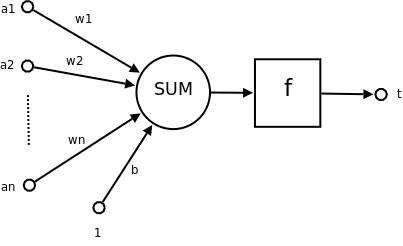
\includegraphics[width=0.8\linewidth]{images/perceptron.png}
		\end{center}
	\end{figure}
	
\subsection{Multilayer Perceptron}
	In order to handle the challenges, some modifications are added into the model.
	
	First, instead of only one layer, more layers are connected to the first layer to form the so called Multilayer Perceptron or Artificial Neural Network. Second, in order to add nonlinearity to fit sophisticated dataset, nonlinear activation function. Activation function is required because without it, the multilayer model will be equivalent to a linear model\cite{goodfellow_bengio_courville_2017}.
	
	\begin{figure}[h]
		\begin{center}
			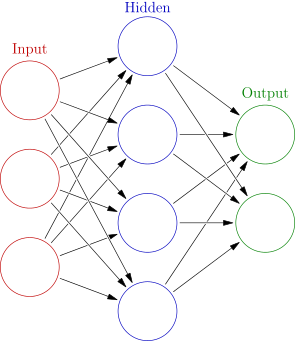
\includegraphics[width=0.5\linewidth]{images/ann}
			\caption{Neural Network}
		\end{center}
	\end{figure}
	
	There are a lot of options for activation function, some of them are listed in the table below.
	
	\begin{figure}[h]
		\begin{center}
			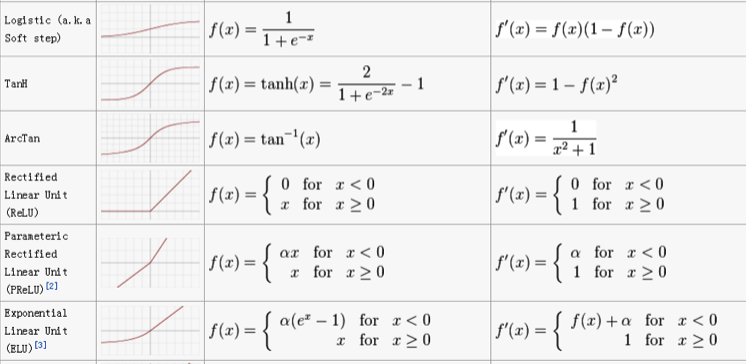
\includegraphics[width=0.8\linewidth]{images/activation}
			\caption{Common Activation Functions}
		\end{center}
	\end{figure}

	The most common activation function is sigmoid, this is a smooth function and is continuously differentiable. The biggest advantage that it has over step and linear function is that it is non-linear\cite{gupta_bansal_srivastava_jain_2017}, and the analytical property of this function is really good that its derivative has a simple closed form.
	
	The tanh function is a scaled version of the sigmoid function, and is symmetric over the origin, so it basically solves our problem of the values all being of the same sign\cite{gupta_bansal_srivastava_jain_2017}.
	
	The big disadvantage of those stair-like functions is that sigmoid can be saturated with large weights and the learning will be slowed down\cite{kotsiantis2007supervised}. To solve this problem, Hinton\cite{kotsiantis2007supervised} proposed to use Rectified Linear Units(ReLU). The main advantage of using the ReLU function over other activation functions is that it does not activate all the neurons at the same time\cite{gupta_bansal_srivastava_jain_2017} because if the input is negative it will convert it to zero and the neuron is not activated.
	
	\begin{figure}[h]
		\begin{center}
			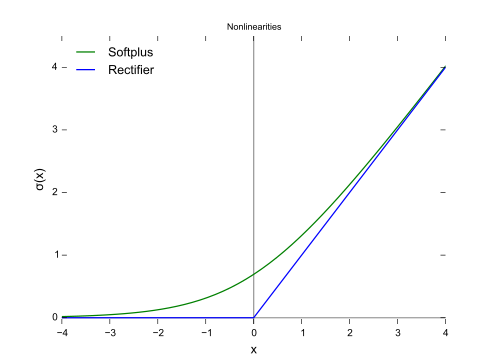
\includegraphics[width=0.8\linewidth]{images/relu}
			\caption{ReLU vs. Softplus}
		\end{center}
	\end{figure}
	
	The problem of ReLU is that when using it, we should be careful because when the activation is trapped by the negative side, since the gradient there is constantly zero, the weights will not be updated anymore. Though this is not a big problem because we can add a small amount to the left side to avoid the problem (Leaky ReLU). Because of the advantages of ReLU, it is still the most popular activation function in Machine Learning community\cite{gupta_bansal_srivastava_jain_2017}.
	
	\subsection{Convolution Neural Network (CNN)}
	Another significant problem of traditional Neural Network is that as the scale of network grows, the number of parameters grows exponentially and thus the convergence will be pretty slow.
	
	Inspired by the research about Receptive fields\cite{hubel1968receptive}, LeCun introduced the well-known LeNet-5 structure\cite{cun_jackel_boser_denker_graf_guyon_henderson_howard_hubbard_1990} to recognize handwritten numbers in MNIST dataset\footnote{http://yann.lecun.com/exdb/mnist/}
	
	\begin{figure}[h]
		\begin{center}
			\includegraphics[width=\linewidth]{images/lenet}
			\caption{LeNet-5}
		\end{center}
	\end{figure}
	
	The symbol of the success of CNN in computer vision is made by the excellent performance made by AlexNet\cite{kotsiantis2007supervised}, GoogLeNet\cite{DBLP:journals/corr/SzegedyLJSRAEVR14} etc. in competitions like ImageNet.
	
	The basic design of CNN are the following:
	
	\begin{enumerate}[(i)]
		\item Shared weights: Shared weights is directly inspired by the idea of Receptive fields. In the network, an input image will be scanned by a window (so called convolution) to generate the next level of feature maps. This gives CNN ability to tolerate translation of the input image. By using only a set of shared weights (filters).
		\item Pooling: Another important design of CNN is pooling, which is a kind of non-linear down-sampling. The intuition is that  the exact location of a feature is less important than its rough location relative to other features\cite{goodfellow_bengio_courville_2017}. Pooling also serves to reduce the spatial size of the represention, which means the number of parameters.
	\end{enumerate}
	
\subsection{Recurrent Neural Network (RNN)}
	While CNN can excellently captures spatial structures, RNN is proposed to dig in sequential and temporal data. They are networks with loops in them, allowing information to persist\cite{colah}
	
	\begin{figure}[h]
		\begin{center}
			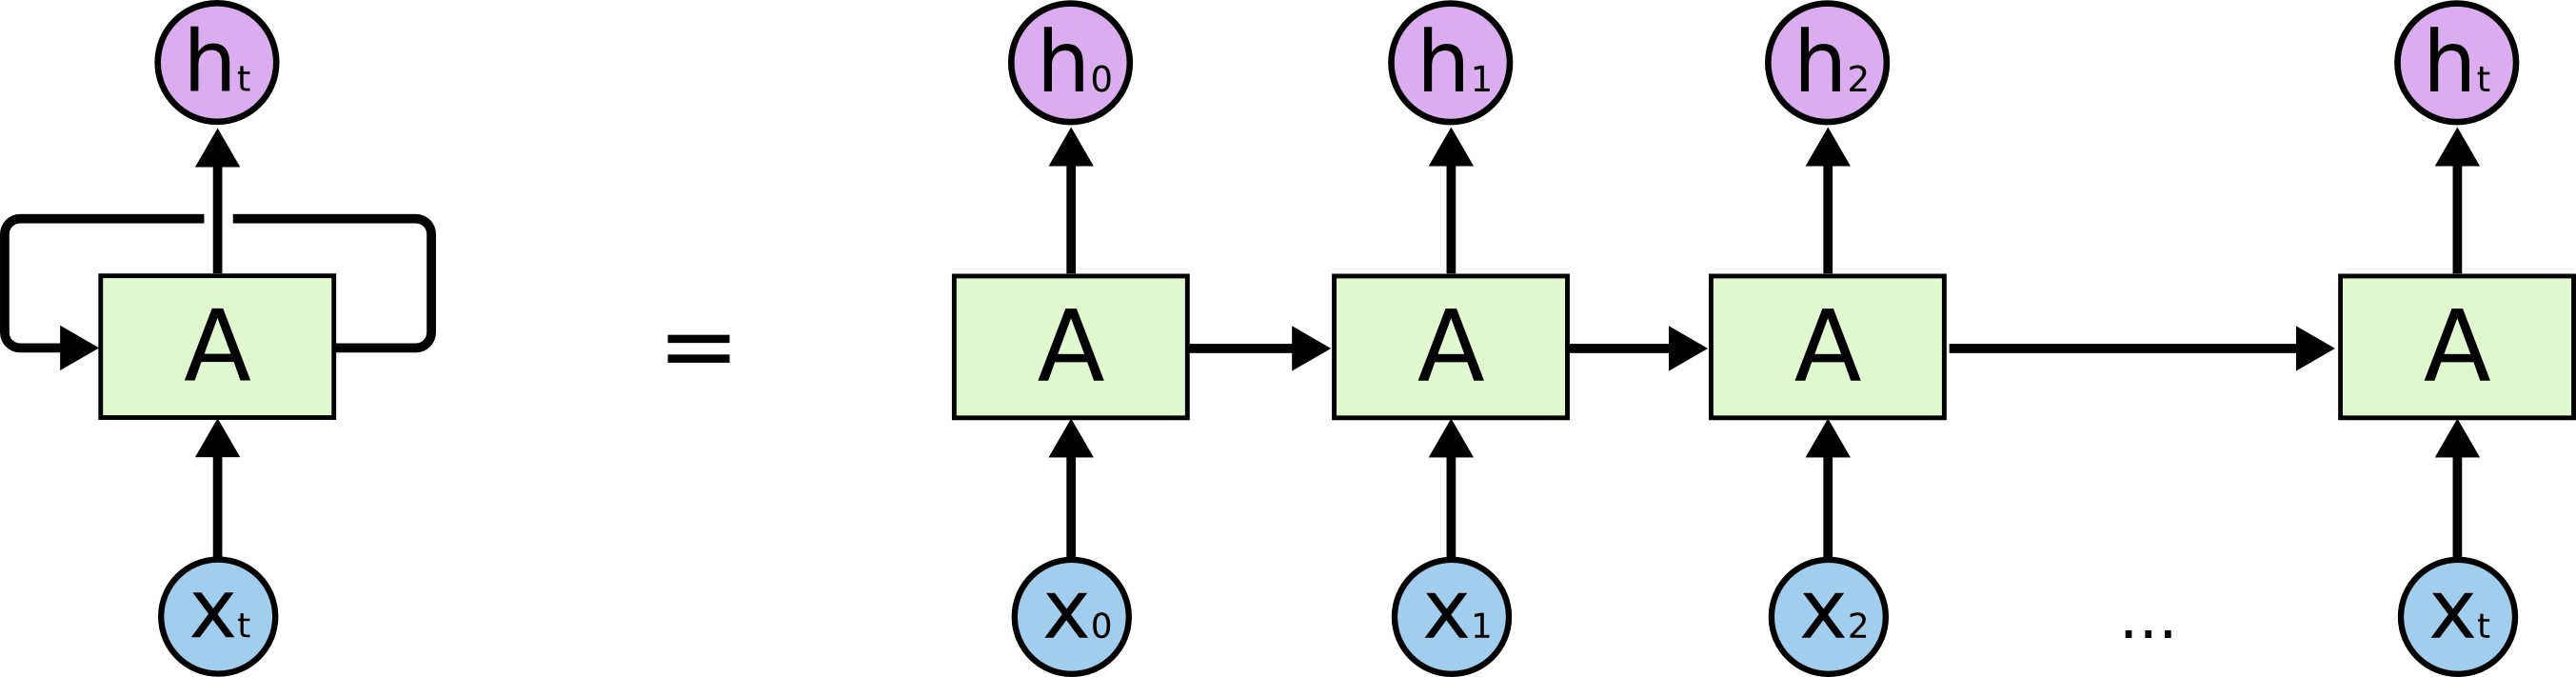
\includegraphics[width=0.8\linewidth]{images/rnn}
			\caption{RNN}
		\end{center}
	\end{figure}

Traditional RNN suffers from problem of gradient explosion and gradient vanishing because of the chain rule of derivative\cite{goodfellow_bengio_courville_2017}. In order to handle this problem and enable the network to detect long-term dependencies, Long Short Term Memory networks(LSTM) is introduced\cite{lstm}. The horizontal line running through the top of the diagram transports the state of cell and input gate and forget gate make the network able to decide which of the information should be remembered and which should be forgot.

	\begin{figure}[h]
		\begin{center}
			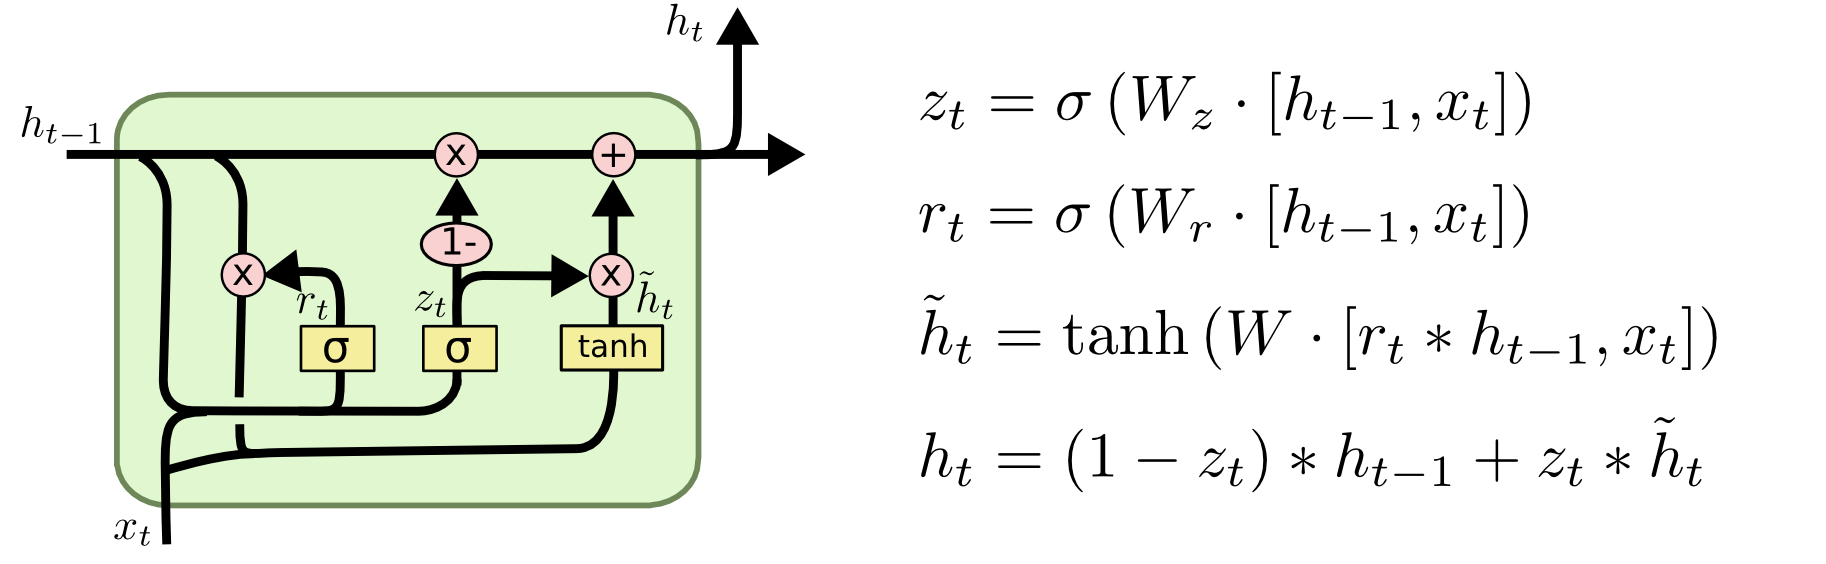
\includegraphics[width=\linewidth]{images/lstm}
			\caption{LSTM}
		\end{center}
	\end{figure}
	
\subsection{Residue Network}
	Just as mention above, as the depth of neural network grows, they became more and more difficult to train due to long dependencies. Kaiming He proposed a residual learning framework to ease the training of networks that are substantially deeper than those used previously\cite{he_zhang_ren_sun_2016}.
	
	\begin{figure}[h]
		\begin{center}
			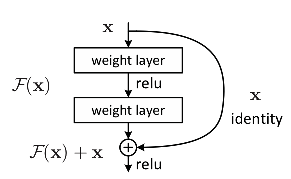
\includegraphics[width=\linewidth]{images/resnet}
			\caption{ResNet\cite{he_zhang_ren_sun_2016}}
		\end{center}
	\end{figure}
	
	By adding the skip structure, the gradient can be passed and maintained to really deep layers and accelerate the training of very massive network. Empirically speaking, the deeper a network is, the more parameters it has, the more capacity the model can show. By solving this problem, massive networks can be trained to solve pretty sophisticated tasks, so the framework became very popular. 
\section{Kernel}
	When data is not linearly separable, another classic trick is to define a kernel function to map the data to a higher dimensional space, where the data can be separated with a hyper-plane.
	
	\begin{figure}[h]
		\begin{center}
			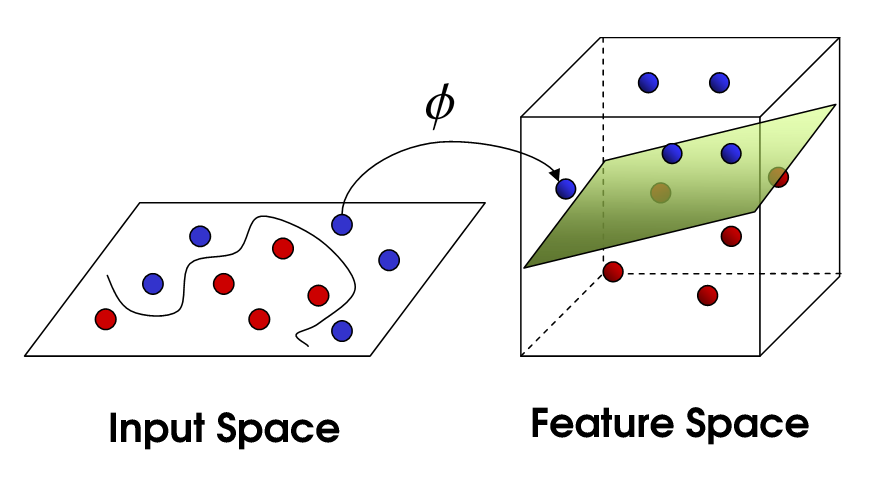
\includegraphics[width=\linewidth]{images/kernel}
			\caption{Kernel Function}\footnote{https://datascience.stackexchange.com/questions/17536/kernel-trick-explanation}
		\end{center}
	\end{figure}
	
	\subsection{Kernel Ridge Regression}
		Recall that in ridge regression, we have our primal problem
		\[L(\mathbf{w}) = (\mathbf{y} - \mathbf{X}\mathbf{w})(\mathbf{y} - \mathbf{X}\mathbf{w}) + \lambda ||\mathbf{w}||^2\]
		
		whose solution is given by 
		
		\[\mathbf{w}^* = (\lambda\mathbf{I} + \mathbf{X}^T\mathbf{X})^{-1}\mathbf{X}^T\mathbf{y}\]
		
		then we can define the the following dual variables
		
		\[\alpha = (\mathbf{K} + \lambda\mathbf{I})\mathbf{y}\]
		
		then we can write
		
		\[\mathbf{w} = \mathbf{X}\mathbf{\alpha}\]
		
		which gives
		
		\[f(\mathbf{x}) = \mathbf{w}^T\mathbf{x} = \sum_{i = 1}^N \alpha_i \kappa(\mathbf{x}, \mathbf{x}_i)\]
		
		The cost of computing the dual variables $\alpha$ is $O(N^3)$, whereas the cost of computing the primal variables $w$ is $O(D^3)$. Hence the kernel method can be useful in high dimensional settings\cite{murphy_2013}. 
		
	\subsection{Support Vector Machine}
	In order to have high robustness, SVM does not only requires the complete separate of data of different labels, but also requires that the hyper-plain can have the maximized decision margin\cite{murphy_2013}. We can convert it to an constrained optimization problem
	
	\[\min_{\mathbf{w}} \frac{1}{2} ||w||^2, s.t. y_i(\mathbf{w}^T\mathbf{x}_i + w_0) \geq 1\]
	
	and sometimes we may which the SVM to have some tolerance, We replace the hard constraints that $y_if_i \geq 0$ with the soft margin constraints that $y_if_i \geq 1 − \xi_i$, so that the optimization problem can become 
	
	\[\min_{\mathbf{w}, \xi} \frac{1}{2} ||w||^2 + C\sum_{i = 1}^N \xi_i, s.t. \xi_i \geq 0, y_i(\mathbf{w}^T\mathbf{x}_i + w_0) \geq 1 - \xi_i\]
	
	Both problems can be solved using SGD, or SMO algorithm\cite{platt1998sequential}.
\section{Instance-based learning}
	Instance-based learning algorithms are lazy-learning algorithms\cite{mitchell_2017} because they delay the induction or generalization process until classification is perform\cite{kotsiantis2007supervised}. Instance-based learning requires little training time but a lot of evaluation time during the process of classification\cite{kotsiantis2007supervised}. The most straight-forward and common example is the nearest neighbor algorithm.
	
	k nearest neighbor algorithm is based on the assumption that spatial closeness leads to categorical similarity, thus it decides the class of a data point by calculating k most close points and make decision by majority vote.
	
	In order to define spatial dissimilarity, metric functions are required. A general metric function $d : M \times M \rightarrow \mathbb{R}$ should satisfy the following requirements:
	
	\begin{enumerate}[(i).]
		\item \[d(x, y) \geq 0\]
		and $d(x,y) = 0$ if and only if $x = y$.
		\item \[d(x,y) = d(y,x)\]
		\item \[d(x,z) \leq d(x,y) + d(y,z)\]
	\end{enumerate}
	
	Commonly used metrics are Minkowsky distance, Euclidean distance etc.\cite{kotsiantis2007supervised}
	
	Computing the nearest neighbor can be really costly when the number of data is large, some data structures are introduced to mitigate this issue. For instance, k-d tree\cite{bentley_1975} is very commonly used to compute nearest neighbor quickly.
\section{Conclusion}
	The review of supervised learning explored all commonly used algorithms and models for classification and regression. By analyzing the pros and cons of each algorithms and present how these models can be fixed to deal with certain challenges, it is reasonable to think this paper presented a relatively detailed guide to researchers on the selection and use of models that are best-known in the domain of supervised learning.

{\small
\bibliographystyle{ieee}
\bibliography{egbib}
}

\end{document}
